% Figura cuerpo B2: el consumo responde a la renta permanente: un impulso fiscal transitorio apenas mueve el consumo
\documentclass[tikz,border=3pt]{standalone}
\usepackage[T1]{fontenc}
\usepackage[utf8]{inputenc}
\usetikzlibrary{arrows.meta,calc,positioning}
\begin{document}
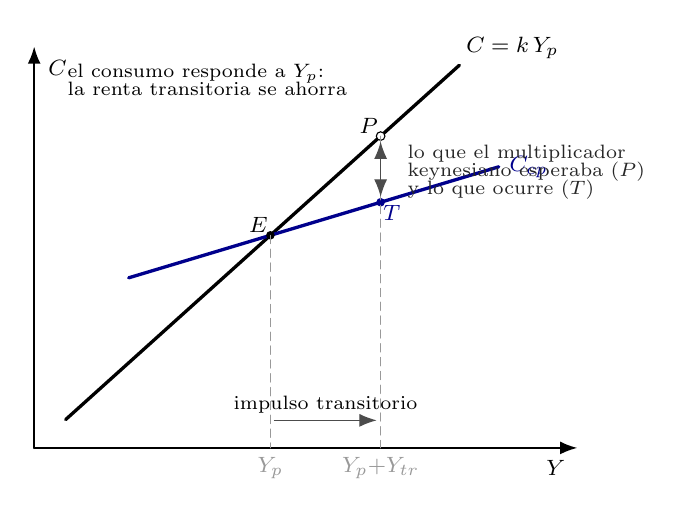
\begin{tikzpicture}[>={Latex[length=2.2mm]}, line cap=round, font=\footnotesize,
  eje/.style={->, thick},
  curva/.style={very thick},
  nueva/.style={very thick, blue!55!black},
  guia/.style={densely dashed, gray!80},
  pto/.style={circle, fill=black, inner sep=1.1pt}]
  \draw[eje] (0,0) -- (6.9,0) node[below left=1pt]{$Y$};
  \draw[eje] (0,0) -- (0,5.1) node[below right=2pt]{$C$};
  % Rayo de largo plazo
  \draw[curva] (0.4,0.36) -- (5.4,4.86) node[above right=-2pt]{$C=k\,Y_p$};
  % Recta de corto plazo (plana)
  \draw[nueva] (1.2,2.16) -- (5.9,3.57) node[right]{$C_{cp}$};
  \node[pto] (E) at (3,2.7) {};
  \node[above left=-2pt of E, inner sep=1pt] {$E$};
  \node[pto, fill=blue!55!black] (T) at (4.4,3.12) {};
  \node[below right=-2pt of T, inner sep=1pt, blue!55!black] {$T$};
  \node[circle, draw=black, fill=white, inner sep=1.1pt] (P) at (4.4,3.96) {};
  \node[above left=-2pt of P, inner sep=1pt] {$P$};
  \draw[guia] (3,2.7) -- (3,0) node[below]{$Y_p$};
  \draw[guia] (4.4,3.96) -- (4.4,0) node[below]{$Y_p{+}Y_{tr}$};
  \draw[->, gray!60!black] (3.05,0.35) -- (4.35,0.35) node[midway, above=-1pt, black]{\scriptsize impulso transitorio};
  \draw[<->, gray!60!black, shorten >=2pt, shorten <=2pt] (4.4,3.12) -- (4.4,3.96);
  \node[align=left, anchor=west, gray!30!black] at (4.62,3.5) {\scriptsize lo que el multiplicador\\[-3pt]\scriptsize keynesiano esperaba ($P$)\\[-3pt]\scriptsize y lo que ocurre ($T$)};
  \node[align=left, anchor=north west] at (0.3,5.0) {\scriptsize el consumo responde a $Y_p$:\\[-3pt]\scriptsize la renta transitoria se ahorra};
\end{tikzpicture}
\end{document}
